\documentclass[tikz]{standalone}

\usepackage{fontspec}

\usetikzlibrary{arrows}
\usetikzlibrary{calc}
\usetikzlibrary{decorations.pathreplacing}
\usetikzlibrary{positioning}
\usetikzlibrary{matrix}

\usepackage{fontspec}

\begin{document}

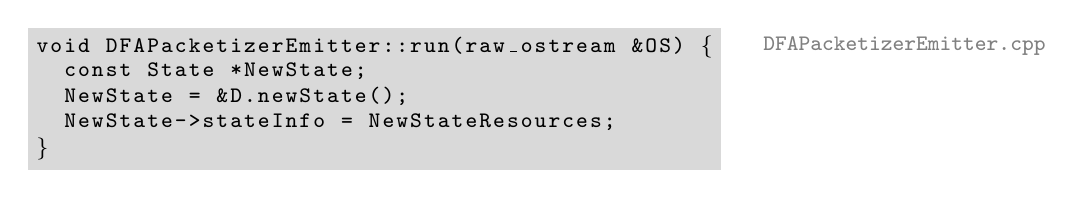
\begin{tikzpicture}
  [node distance=5mm, >=stealth',
  every node/.style={font=\footnotesize},
  every matrix/.style={fill=black!15, inner sep=1mm, row sep=0.5mm,
                        matrix of nodes, nodes in empty cells,
                        minimum height=0.5em, minimum width=.5em,
                        nodes={anchor=base, inner sep=0, font=\ttfamily\footnotesize}}]

  \matrix (snippet) {
v & o & i & d &   & D & F & A & P & a & c & k & e & t & i & z & e & r & E & m & i & t & t & e & r & : & : & r & u & n & ( & r & a & w & \_ & o & s & t & r & e & a & m &   & \& & O & S & ) &   & \{ \\
  &   & c & o & n & s & t &   & S & t & a & t & e &   & * & N & e & w & S & t & a & t & e & ; &   &   &   &   &   &   &   &   &   &   &   &   &   &   &   &   &   &   &   &   &   &   &   &   &   \\
  &   & N & e & w & S & t & a & t & e &   & = &   & \& & D & . & n & e & w & S & t & a & t & e & ( & ) & ; &   &   &   &   &   &   &   &   &   &   &   &   &   &   &   &   &   &   &   &   &   &   \\
  &   & N & e & w & S & t & a & t & e & - & > & s & t & a & t & e & I & n & f & o &   & = &   & N & e & w & S & t & a & t & e & R & e & s & o & u & r & c & e & s & ; &   &   &   &   &   &   &   \\
\} &   &   &   &   &   &   &   &   &   &   &   &   &   &   &   &   &   &   &   &   &   &   &   &   &   &   &   &   &   &   &   &   &   &   &   &   &   &   &   &   &   &   &   &   &   &   &   &   \\
  };
 \node [above, anchor=west, black!50, xshift=0.5cm]
        at (snippet-1-49.east)
        {\texttt{DFAPacketizerEmitter.cpp}};
\end{tikzpicture}

\end{document}
